%% (Master) Thesis template
% Template version used: v1.4
%
% Largely adapted from Adrian Nievergelt's template for the ADPS
% (lecture notes) project.


%% We use the memoir class because it offers a many easy to use features.
\documentclass[11pt,a4paper,titlepage]{memoir}

%% Packages
%% ========

%% LaTeX Font encoding -- DO NOT CHANGE
\usepackage[OT1]{fontenc}

%% Babel provides support for languages.  'english' uses British
%% English hyphenation and text snippets like "Figure" and
%% "Theorem". Use the option 'ngerman' if your document is in German.
%% Use 'american' for American English.  Note that if you change this,
%% the next LaTeX run may show spurious errors.  Simply run it again.
%% If they persist, remove the .aux file and try again.
\usepackage[english]{babel}

%% Input encoding 'utf8'. In some cases you might need 'utf8x' for
%% extra symbols. Not all editors, especially on Windows, are UTF-8
%% capable, so you may want to use 'latin1' instead.
\usepackage[utf8]{inputenc}

%% This changes default fonts for both text and math mode to use Herman Zapfs
%% excellent Palatino font.  Do not change this.
\usepackage[sc]{mathpazo}

%% The AMS-LaTeX extensions for mathematical typesetting.  Do not
%% remove.
\usepackage{amsmath,amssymb,amsfonts,mathrsfs}

%% NTheorem is a reimplementation of the AMS Theorem package. This
%% will allow us to typeset theorems like examples, proofs and
%% similar.  Do not remove.
%% NOTE: Must be loaded AFTER amsmath, or the \qed placement will
%% break
\usepackage[amsmath,thmmarks]{ntheorem}

%% LaTeX' own graphics handling
\usepackage{graphicx}

%% We unfortunately need this for the Rules chapter.  Remove it
%% afterwards; or at least NEVER use its underlining features.
\usepackage{soul}

%% This allows you to add .pdf files. It is used to add the
%% declaration of originality.
\usepackage{pdfpages}

%% Some more packages that you may want to use.  Have a look at the
%% file, and consult the package docs for each.
%% See the TeXed file for more explanations

%% [OPT] Multi-rowed cells in tabulars
%\usepackage{multirow}

%% [REC] Intelligent cross reference package. This allows for nice
%% combined references that include the reference and a hint to where
%% to look for it.
\usepackage{varioref}

%% [OPT] Easily changeable quotes with \enquote{Text}
%\usepackage[german=swiss]{csquotes}

%% [REC] Format dates and time depending on locale
\usepackage{datetime}

%% [OPT] Provides a \cancel{} command to stroke through mathematics.
%\usepackage{cancel}

%% [NEED] This allows for additional typesetting tools in mathmode.
%% See its excellent documentation.
\usepackage{mathtools}

%% [ADV] Conditional commands
%\usepackage{ifthen}

%% [OPT] Manual large braces or other delimiters.
%\usepackage{bigdelim, bigstrut}

%% [REC] Alternate vector arrows. Use the command \vv{} to get scaled
%% vector arrows.
\usepackage[h]{esvect}

%% [NEED] Some extensions to tabulars and array environments.
\usepackage{array}

%% [OPT] Postscript support via pstricks graphics package. Very
%% diverse applications.
%\usepackage{pstricks,pst-all}

%% [?] This seems to allow us to define some additional counters.
%\usepackage{etex}

%% [ADV] XY-Pic to typeset some matrix-style graphics
%\usepackage[all]{xy}

%% [OPT] This is needed to generate an index at the end of the
%% document.
%\usepackage{makeidx}

%% [OPT] Fancy package for source code listings.  The template text
%% needs it for some LaTeX snippets; remove/adapt the \lstset when you
%% remove the template content.
\usepackage{listings}
\lstset{language=TeX,basicstyle={\normalfont\ttfamily}}

%% [REC] Fancy character protrusion.  Must be loaded after all fonts.
\usepackage{microtype}

%% [REC] Nicer tables.  Read the excellent documentation.
\usepackage{booktabs}

\usepackage{tikz}

%% Our layout configuration.  DO NOT CHANGE.
%% Memoir layout setup

%% NOTE: You are strongly advised not to change any of them unless you
%% know what you are doing.  These settings strongly interact in the
%% final look of the document.

% Dependencies
\usepackage{ETHlogo}

% Turn extra space before chapter headings off.
\setlength{\beforechapskip}{0pt}

\nonzeroparskip
\parindent=0pt
\defaultlists

% Chapter style redefinition
\makeatletter

\if@twoside
  \pagestyle{Ruled}
  \copypagestyle{chapter}{Ruled}
\else
  \pagestyle{ruled}
  \copypagestyle{chapter}{ruled}
\fi
\makeoddhead{chapter}{}{}{}
\makeevenhead{chapter}{}{}{}
\makeheadrule{chapter}{\textwidth}{0pt}
\copypagestyle{abstract}{empty}

\makechapterstyle{bianchimod}{%
  \chapterstyle{default}
  \renewcommand*{\chapnamefont}{\normalfont\Large\sffamily}
  \renewcommand*{\chapnumfont}{\normalfont\Large\sffamily}
  \renewcommand*{\printchaptername}{%
    \chapnamefont\centering\@chapapp}
  \renewcommand*{\printchapternum}{\chapnumfont {\thechapter}}
  \renewcommand*{\chaptitlefont}{\normalfont\huge\sffamily}
  \renewcommand*{\printchaptertitle}[1]{%
    \hrule\vskip\onelineskip \centering \chaptitlefont\textbf{\vphantom{gyM}##1}\par}
  \renewcommand*{\afterchaptertitle}{\vskip\onelineskip \hrule\vskip
    \afterchapskip}
  \renewcommand*{\printchapternonum}{%
    \vphantom{\chapnumfont {9}}\afterchapternum}}

% Use the newly defined style
\chapterstyle{bianchimod}

\setsecheadstyle{\Large\bfseries\sffamily}
\setsubsecheadstyle{\large\bfseries\sffamily}
\setsubsubsecheadstyle{\bfseries\sffamily}
\setparaheadstyle{\normalsize\bfseries\sffamily}
\setsubparaheadstyle{\normalsize\itshape\sffamily}
\setsubparaindent{0pt}

% Set captions to a more separated style for clearness
\captionnamefont{\sffamily\bfseries\footnotesize}
\captiontitlefont{\sffamily\footnotesize}
\setlength{\intextsep}{16pt}
\setlength{\belowcaptionskip}{1pt}

% Set section and TOC numbering depth to subsection
\setsecnumdepth{subsection}
\settocdepth{subsection}

%% Titlepage adjustments
\pretitle{\vspace{0pt plus 0.7fill}\begin{center}\HUGE\sffamily\bfseries}
\posttitle{\end{center}\par}
\preauthor{\par\begin{center}\let\and\\\Large\sffamily}
\postauthor{\end{center}}
\predate{\par\begin{center}\Large\sffamily}
\postdate{\end{center}}

\def\@advisors{}
\newcommand{\advisors}[1]{\def\@advisors{#1}}
\def\@department{}
\newcommand{\department}[1]{\def\@department{#1}}
\def\@thesistype{}
\newcommand{\thesistype}[1]{\def\@thesistype{#1}}

\renewcommand{\maketitlehooka}{\noindent\ETHlogo[2in]}

\renewcommand{\maketitlehookb}{\vspace{1in}%
  \par\begin{center}\Large\sffamily\@thesistype\end{center}}

\renewcommand{\maketitlehookd}{%
  \vfill\par
  \begin{flushright}
    \sffamily
    \@advisors\par
    \@department, ETH Z\"urich
  \end{flushright}
}

\checkandfixthelayout

\setlength{\droptitle}{-48pt}

\makeatother

% This defines how theorems should look. Best leave as is.
\theoremstyle{plain}
\setlength\theorempostskipamount{0pt}

%%% Local Variables:
%%% mode: latex
%%% TeX-master: "thesis"
%%% End:


%% Theorem environments.  You will have to adapt this for a German
%% thesis.
%% Theorem-like environments

%% This can be changed according to language. You can comment out the ones you
%% don't need.

\numberwithin{equation}{chapter}

%% German theorems
%\newtheorem{satz}{Satz}[chapter]
%\newtheorem{beispiel}[satz]{Beispiel}
%\newtheorem{bemerkung}[satz]{Bemerkung}
%\newtheorem{korrolar}[satz]{Korrolar}
%\newtheorem{definition}[satz]{Definition}
%\newtheorem{lemma}[satz]{Lemma}
%\newtheorem{proposition}[satz]{Proposition}

%% English variants
\newtheorem{theorem}{Theorem}[chapter]
\newtheorem{example}[theorem]{Example}
\newtheorem{remark}[theorem]{Remark}
\newtheorem{corollary}[theorem]{Corollary}
\newtheorem{definition}[theorem]{Definition}
\newtheorem{lemma}[theorem]{Lemma}
\newtheorem{proposition}[theorem]{Proposition}

%% Proof environment with a small square as a "qed" symbol
\theoremstyle{nonumberplain}
\theorembodyfont{\normalfont}
\theoremsymbol{\ensuremath{\square}}
\newtheorem{proof}{Proof}
%\newtheorem{beweis}{Beweis}


%% Helpful macros.
%% Custom commands
%% ===============

%% Special characters for number sets, e.g. real or complex numbers.
\newcommand{\C}{\mathbb{C}}
\newcommand{\K}{\mathbb{K}}
\newcommand{\N}{\mathbb{N}}
\newcommand{\Q}{\mathbb{Q}}
\newcommand{\R}{\mathbb{R}}
\newcommand{\Z}{\mathbb{Z}}
\newcommand{\X}{\mathbb{X}}

%% Fixed/scaling delimiter examples (see mathtools documentation)
\DeclarePairedDelimiter\abs{\lvert}{\rvert}
\DeclarePairedDelimiter\norm{\lVert}{\rVert}

%% Use the alternative epsilon per default and define the old one as \oldepsilon
\let\oldepsilon\epsilon
\renewcommand{\epsilon}{\ensuremath\varepsilon}

%% Also set the alternate phi as default.
\let\oldphi\phi
\renewcommand{\phi}{\ensuremath{\varphi}}

\DeclareMathOperator{\dgm}{Dgm}

\newcommand{\todo}[1]{\textcolor{red}{TODO: #1}}

%% Make document internal hyperlinks wherever possible. (TOC, references)
%% This MUST be loaded after varioref, which is loaded in 'extrapackages'
%% above.  We just load it last to be safe.
\usepackage[linkcolor=black,colorlinks=true,citecolor=black,filecolor=black]{hyperref}


%% Document information
%% ====================

\title{Persistence of generalised density functions}
\author{Maxim Mikhaylov}
\thesistype{Master Thesis}
\advisors{Supervisors: Prof.\ Dr.\ B. G\"artner, Dr.\ P. Schnider}
\department{Department of Computer Science}
\date{June 30, 2025}

\begin{document}

\frontmatter

%% Title page is autogenerated from document information above.  DO
%% NOT CHANGE.
\begin{titlingpage}
  \calccentering{\unitlength}
  \begin{adjustwidth*}{\unitlength-24pt}{-\unitlength-24pt}
    \maketitle
  \end{adjustwidth*}
\end{titlingpage}

%% The abstract of your thesis.  Edit the file as needed.
\begin{abstract}
    Topological data analysis (TDA) often uses density-like functions defined on
    the ambient space $\R^d$ to infer the underlying topological structure of a
    dataset $P \subseteq \R^d$. The persistent homology of the sublevelset or
    superlevelset filtrations induced by these functions captures multi-scale
    topological features. A key desirable property is \emph{stability}: small
    perturbations in the dataset result in similarly small changes in the
    persistence diagrams. A classic example is the nearest-neighbour distance
    function $f_{\operatorname{dist}}(P, x) \coloneqq \min_{p\in P} d(x, p)$,
    whose sublevel sets are homotopy equivalent to the \v{C}ech
    complex~\cite{schnider2024introduction}, for which the bottleneck
    distance between persistence diagrams $\dgm(f_P)$ and $\dgm(f_Q)$ is
    bounded by the Hausdorff distance $d_H(P, Q)$ between datasets
    \cite{chazal2013persistencestabilitygeometriccomplexes}:
    \[d_b(\dgm(f_P), \dgm(f_Q)) \leq d_H(P, Q).\]
    This thesis investigates \emph{generalised density functions}, which are
    functions $f : \mathcal{P}(\R^d) \times \R^d \to \R$, where
    $\mathcal{P}(\R^d)$ denotes the set of all finite subsets of $\R^d$, and
    the conditions under which they satisfy a stability property of the form
    \[d_b(\dgm(f_P), \dgm(f_Q)) \leq c \cdot d_H(P, Q)\]
    for some finite constant $c$.

    The primary contributions of this work are stability theorems for several
    classes of generalised density functions. Specifically, we prove stability
    bounds for:
    \begin{itemize}
        \item Several generalisations of the nearest-neighbour distance function
            of the form $f(P, x) = \min_{p\in P} h(x, p)$.
        \item Functions that are Lipschitz continuous with respect to the
            Hausdorff distance on the space of point clouds.
        \item Morse functions that satisfy a Lipschitz-like condition.
    \end{itemize}

    Beyond these core stability results, we explore the properties of the space
    of stable functions and investigate how common operations, such as addition
    and taking minima, affect stability. We identify conditions under which
    stability is preserved under these operations and provide counterexamples
    demonstrating cases where it is not.
    
    Our findings unify and extend existing stability results, offering practical
    guidance for the selection and design of generalised density functions for
    topological data analysis.
\end{abstract}


%% TOC with the proper setup, do not change.
\cleartorecto
\tableofcontents
\mainmatter

%% Your real content!
% Some commands used in this file
\newcommand{\package}{\emph}

\chapter{Introduction}
\label{chap:introduction}

Topological Data Analysis (TDA) provides a robust framework for understanding
the shape of data. Among its tools is \emph{persistent homology}, which extracts
topological features across different scales. Traditionally, persistent homology
is applied to a finite point cloud $P \subseteq X$ through filtrations of
simplicial complexes built on top of $P$, such as the Vietoris–Rips or \v{C}ech
complexes. An alternative (though sometimes equivalent) approach involves
defining a real-valued function $X \to \R$ that encodes the geometry of the
data, and then computing the persistent homology of its sublevel (or superlevel)
set filtration. The resulting persistent homology captures topological features
such as connected components, loops, and voids, and encodes them in a
persistence diagram, which summarizes their birth and death across the
filtration.

A classical and widely studied example is the \emph{nearest-neighbor distance
function},
\begin{equation}
    f(P, x) = \min_{p \in P} d(x, p),
\end{equation}
where $d$ is a metric on $X$. The homology groups of the sublevel set filtration
of this function are precisely the homology groups of the \v{C}ech filtration.
This function satisfies a \emph{stability} property:
\begin{equation}
    d_b(\dgm_{f(P)}, \dgm_{f(Q)}) \leq d_H(P, Q),
\end{equation}
where $d_b$ is the bottleneck distance between persistence diagrams and $d_H$ is
the Hausdorff distance between point clouds.
Stability ensures that small perturbations in the data lead to proportionally
small changes in the persistence diagrams, guaranteeing that the topological
features extracted from the data are robust to noise.

However, the nearest-neighbor function is just one of many possible density-like
functions for TDA. In practice, alternative functions may offer computational
advantages, better capture intrinsic structure, or incorporate domain knowledge.
For example, the DTM filtration~\cite{anai2020dtm} modifies the nearest-neighbor
function to make it more robust to noise and outliers. This motivates the study
of \emph{generalized density functions}, which are functions of the form
\begin{equation}
    f(P, x) : \mathcal{P}(X) \times X \to \R.
\end{equation}
For a given point cloud $P$, such a function defines a real-valued function
$f_P: X \to \R$, whose sublevel set filtration can be used to analyze the
topological features of $P$. We say $f$ is $c$-\emph{stable} if for all point
clouds $P, Q \subseteq X$ we have
\begin{equation}
    d_b(\dgm_{f(P)}, \dgm_{f(Q)}) \leq c \cdot d_H(P, Q),
\end{equation}
where the constant $c$ measures the sensitivity of the persistence diagrams to
perturbations in the data.

In this thesis, we investigate which functions are stable. We consider the
following classes of functions:
\begin{enumerate}
    \item Functions of the form $f(P, x) = \min_{p \in P} h(d(p, x))$, where $h$
          is a monotone Lipschitz continuous function. These generalize the
          classical nearest-neighbor function while preserving stability.
    \item Further generalization to $f(P, x) = \min_{p \in P} h(p, x)$, where
          $h$ is a Lipschitz function with respect to $p$.
    \item Functions $f(P, x)$ that are Lipschitz with respect to point clouds
          \emph{(PC-Lipschitz)}, where $\mathcal{P}(X)$ is equipped with the
          Hausdorff distance, and the space of real-valued functions $f_P : X
          \to \R$ is equipped with the $L_\infty$-norm.
    \item Finally, we consider Morse functions whose restriction to the critical
          points is Lipschitz continuous.
\end{enumerate}

Beyond these classes, we also study when stability is preserved under common
operations. For example, if two functions are each stable, under what conditions
is their pointwise minimum or average also stable? We identify sufficient
conditions and provide concrete counterexamples demonstrating cases where
stability fails. This analysis shows how more complex stable functions can be
constructed from simpler ones, and provides insight into the structure of the
space of stable functions.

Finally, we examine the topological and algebraic properties of the space of
$c$-stable functions itself. We analyze properties such as convexity,
contractibility, and closedness, as well as establish a lattice structure on the
set of $c$-PC-Lipschitz functions.

Taken together, our results contribute to the theoretical foundations of TDA by
deepening the understanding of stability for generalized density functions. They
also provide practical guidance for designing stable filtrations.

\section{Overview}

The remainder of this thesis is organized as follows:
\begin{itemize}
    \item Chapter~\ref{chap:background} provides the necessary background on
        persistent homology, stability, as well as known stability results.
    \item Chapter~\ref{chap:stable_functions} presents our main contributions:
        stability theorems for various classes of generalized density functions.
    \item Chapter~\ref{chap:operations} studies stability under common
        operations.
    \item Chapter~\ref{chap:space} explores the properties of the space of
        $c$-stable functions, including its topological and algebraic
        structure.
    \item Chapter~\ref{chap:conclusion} concludes with directions for future
        work and open questions.
\end{itemize}

\chapter{Background}
\label{chap:background}

This chapter reviews the mathematical foundations for stability of generalized
density functions. We briefly review the core concepts of how real-valued
functions induce filtrations for persistent homology and then focus on
established stability theorems that serve as a foundation and motivation for
this work. We assume the reader has a working knowledge of topological data
analysis, mainly persistent homology.

\section{Generalized density functions and filtrations}

At the heart of this thesis lies the concept of a generalized density function (GDF).
\begin{definition}[Generalized density function]
    A generalized density function is a map $f : \mathcal{P}(X) \times X \to \R$,
    where $\mathcal{P}(X)$ denotes the power set of $X$. For a given point cloud
    $P \in \mathcal{P}(X)$, a GDF $f$ induces a real-valued function $f_P : X
    \to \R$ defined by $f_P(x) \coloneqq f(P, x)$.
\end{definition}

These functions $f_P$ are used to construct \emph{sublevel set filtrations}.
\begin{definition}[Sublevel set filtration]
    Given a function $f_P : X \to \R$, its sublevel set at a value $a \in \R$ is
    \begin{equation}
        f_P^{-1}(-\infty, a] = \{ x \in X \mid f_P(x) \leq a \}.
    \end{equation}
    The sublevel set filtration of $g$ is the nested family of sets
    $\{f_P^{-1}(-\infty, a]\}_{a \in \R}$.
\end{definition}
Alternatively, superlevel set filtrations can be used, which are defined by
$\{f_P^{-1}[a, +\infty)\}_{a \in \R}$. The choice between sublevel and superlevel
set filtrations is a matter of convention, as the superlevel set filtration of
$f_P$ is exactly the sublevel set filtration of the function $-f_P$, and vice
versa. For the sake of consistency, we will use sublevel set filtrations
throughout this thesis.

Applying a homology functor $H_k$ to the filtration $\{f_P^{-1}(-\infty, a]\}_{a \in \R}$
yields a persistence module, which tracks the evolution of topological features
as the parameter $a$ varies. The \emph{persistence diagram}, denoted $\dgm_k(f_P)$,
is a multiset of points $(b_i, d_i)$ in the extended plane $\overline{\R}^2$,
where $b_i$ represents the birth time and $d_i$ the death time of a
$k$-dimensional feature. An example of a persistence diagram is shown in
Figure~\ref{fig:pd}.

\begin{figure}
    \centering
    \begin{tikzpicture}
        \small
        % Axes
        \draw[->] (0,0) -- (5,0) node[right] {Birth};
        \draw[->] (0,0) -- (0,5.5) node[above] {Death};
        
        % Grid
        % \draw[gray!30] (0,0) grid (6,6);
        
        % Diagonal
        \draw[dashed] (0,0) -- (5,5);
        
        % Point coords
        \coordinate (p1) at (1,3);
        \coordinate (p2) at (2,4);
        \coordinate (p3) at (1.5,2);
        \coordinate (p4) at (3,5);
        
        % Lines to axes
        \draw[dashed,gray] (p1) -- (1,0) node[below,black] {$b_1$};
        \draw[dashed,gray] (p1) -- (0,3) node[left,black] {$d_1$};
        \draw[dashed,gray] (p2) -- (2,0) node[below,black] {$b_2$};
        \draw[dashed,gray] (p2) -- (0,4) node[left,black] {$d_2$};
        \draw[dashed,gray] (p3) -- (1.5,0) node[below,black] {$b_3$};
        \draw[dashed,gray] (p3) -- (0,2) node[left,black] {$d_3$};
        \draw[dashed,gray] (p4) -- (3,0) node[below,black] {$b_4$};
        \draw[dashed,gray] (5,5) -- (0,5) node[left,black] {$\infty$};

        % Points
        \fill (p1) circle (2pt) node[above right] {$p_1$};
        \fill (p2) circle (2pt) node[above right] {$p_2$};
        \fill (p3) circle (2pt) node[above right] {$p_3$};
        \fill (p4) circle (2pt) node[above right] {$p_4$};
    \end{tikzpicture}
    \caption{An example of a persistent diagram. A point $p_i$ is born at $b_i$ and dies at $d_i$. The point $p_4$ does not die, so its death time is
    $\infty$. The dashed line indicates the diagonal $\Delta$, where $b_i = d_i$.}
    \label{fig:pd}
\end{figure}

\section{Quantifying stability}

To formalize the notion of stability, we need metrics to compare both point
clouds and persistence diagrams. A common metric for point clouds is the
\emph{Hausdorff distance}, which is also used in the definition of stability of
the nearest-neighbor distance function.
\begin{definition}[Hausdorff distance]
    Given two non-empty sets $P, Q \subseteq X$, where $X$ is a metric space,
    the Hausdorff distance between $P$ and $Q$ is defined as
    \begin{equation}
        d_H(P, Q) = \max\left\{ \sup_{p \in P} \inf_{q \in Q} d(p, q), \sup_{q \in Q} \inf_{p \in P} d(q, p) \right\}.
    \end{equation}
\end{definition}
Intuitively, the Hausdorff distance measures the ``maximum mismatch'' between the two
sets, capturing the largest distance between a point in one set and its closest
neighbor in the other set.
% It should be noted that for arbitrary $P, Q \subseteq X$, the
% Hausdorff distance may be infinite, which makes it not a metric. However, if we
% assume that $P$ and $Q$ are not empty and compact, then the Hausdorff distance is
% a metric.
% \todo{reword for flow}
% This assumption is reasonable in the context of TDA, where we typically work with
% finite non-empty point clouds.

As the Hausdorff distance requires $X$ to be a metric space, we will assume this
throughout the thesis.

\begin{definition}[Bottleneck distance]
    Given two persistence diagrams $D_1$ and $D_2$, the bottleneck distance
    between them is defined as
    \begin{equation}
        d_b(D_1, D_2) = \inf_\pi \sup_{(b, d) \in D_1} \norm{(b, d) - \pi(b, d)}_\infty,
    \end{equation}
    where the infimum is taken over all bijections $\pi$ between $D_1$ and
    $D_2$, allowing for the possibility of matching points to the diagonal $\Delta = \{(x, x) \mid x \in \overline{\R}\}$.
\end{definition}
The bottleneck distance measures the cost of the ``most expensive'' matching
between the points of the two diagrams, where the cost is defined as the longest
edge in the matching.

% A generalization of the bottleneck distance is the \emph{Wasserstein distance},
% which defines the cost of matching points in terms of the $p$-norm:
% \begin{definition}[Wasserstein distance]
%     Given two persistence diagrams $D_1$ and $D_2$, the Wasserstein distance
%     between them is defined as
%     \begin{equation}
%         d_p(D_1, D_2) = \inf_\pi \left( \sum_{(b, d) \in D_1} \norm{(b, d) - \pi(b, d)}^p_\infty \right)^{1/p},
%     \end{equation}
%     where the infimum is taken over the same bijections $\pi$ as in the
%     bottleneck distance.
% \end{definition}
% The case $p = \infty$ corresponds to the bottleneck distance.
% \todo{possibly remove, if Wasserstein distance isn't used later}

With these metrics, we can formally define stability for a GDF.
\begin{definition}
    A generalized density function $f : \mathcal{P}(X) \times X \to \R$ is
    $c$-\emph{stable} if for all non-empty finite point clouds $P, Q \subseteq
    X$ and all homology dimensions $k \geq 0$, we have
    \begin{equation}
        d_b(\dgm_k(f_P), \dgm_k(f_Q)) \leq c \cdot d_H(P, Q).
    \end{equation}
    If no such finite $c$ exists, we say that $f$ is \emph{unstable} or
    $\infty$-stable.
\end{definition}

\section{Known stability results}

This section reviews the known stability results for GDFs and simplicial
filtrations that can be represented as GDFs.

\subsection{\v{C}ech filtration}
As mentioned in Chapter~\ref{chap:introduction}, the \v{C}ech filtration can be
represented as the sublevel set filtration of the nearest-neighbor distance
function $f_{\mathrm{dist}}(P, x) \coloneqq \min_{p\in P} d(x, p)$.
The sublevel sets $f_{\mathrm{dist}, P}^{-1}(-\infty, a]$ are precisely
$\bigcup_{p\in P} B(p, a)$, the union of closed balls of radius $a$ centered at
the points of $P$. The nerve of this union of balls defines the \v{C}ech
complex. By the Nerve theorem~\cite{Borsuk1948,leray1945forme}, if $P$ is finite,
the \v{C}ech complex is homotopy equivalent to the union of balls.

The stability of this construction is a well-known result:
\begin{theorem}[Stability of the \v{C}ech filtration, \cite{chazal2013persistencestabilitygeometriccomplexes}]
    Let $f_{\mathrm{dist}, P}(x) \coloneqq \min_{p\in P} d(x, p)$. Then for all finite
    $P, Q \subseteq \mathcal{P}(X)$ and any dimension $k \geq 0$, we have
    \begin{equation}
        d_b(\dgm_k(f_{\mathrm{dist}, P}), \dgm_k(f_{\mathrm{dist}, Q})) \leq d_H(P, Q).
    \end{equation}
\end{theorem}
Using the terminology of this thesis, we say the nearest-neighbor distance
function is 1-stable.

\subsection{Weighted \v{C}ech filtration}

The weighted \v{C}ech filtration is a generalization of the \v{C}ech filtration
used to define the DTM-filtration~\cite{anai2020dtm}.

\begin{definition}[Weighted \v{C}ech filtration]
    Let $X = \R^d$, $q \in [1, \infty)$, $P \subseteq \R^d$ and
    $g : P \to \R_{\geq 0}$. For every $p \in P, a \in \R^+$, we define the
    function $r_p(a)$ to be:
    \begin{equation}
        r_p^{(q)}(a) = \begin{cases}
            - \infty, & \text{if } a < g(p), \\
            (a^q - g(p)^q)^{1/q}, & \text{otherwise}.
        \end{cases}
    \end{equation}
    For $q = \infty$, we also define
    \begin{equation}
        r_p^{(q)}(a) = \begin{cases}
            - \infty, & \text{if } a < g(p), \\
            a, & \text{otherwise}.
        \end{cases}
    \end{equation}
    $g(p)$ acts as a weight for each point $p \in P$, influencing the radius
    $r_p^{(q)}(a)$ of the ball $B(p, r_p^{(q)}(a))$. Concretely, the weighted
    \v{C}ech filtration is defined as
    \begin{equation}
        V^a_q[P, g] = \bigcup_{p \in P} B(p, r_p^{(q)}(a)),
    \end{equation}
    where the balls are closed, and the ball of radius $-\infty$ is the empty
    set.
\end{definition}
The weighted \v{C}ech filtration is a strict generalization of the \v{C}ech
filtration, as the \v{C}ech filtration is the special case where $g(p) = 0$ for
all $p \in P$.

Similarly to the \v{C}ech filtration, this filtration can be represented as a
GDF of the form
\begin{equation}
    f_{g, q}(P, x) = \min_{p \in P} (d(x, p)^{q} + g(p)^{q})^{1/q},
\end{equation}
where similarly to the $L_\infty$-norm, when $q = \infty$, the term
$(d(x, p)^q + g(p)^q)^{1/q}$ is replaced by $\max(d(x, p), g(p))$.
A proof of the equivalence of this GDF and the weighted \v{C}ech filtration is
given in Appendix~\ref{app:weighted_cech}.

If $g$ is Lipschitz continuous, then the weighted \v{C}ech filtration is stable:
\begin{theorem}[Stability of the weighted \v{C}ech filtration, \cite{anai2020dtm}]
    Let $P, Q \subset \R^n$ be compact and $g : P \cup Q \to \R^+$ be a
    Lipschitz continuous function with Lipschitz constant $c$. Then for any
    dimension $k \geq 0$, we have
    \begin{equation}
        d_b(\dgm_k(V^a_q[P, g]), \dgm_k(V^a_q[Q, g])) \leq (1 + c^q)^{1/q} \cdot d_H(P, Q),
    \end{equation}
\end{theorem}
This theorem immediately implies that the corresponding GDF
is $(1 + c^q)^{1/q}$-stable.

\subsection{Stability of $L_\infty$-norm-bounded functions}

This fundamental result relates the bottleneck distance between persistence
diagrams of two functions to the $L_\infty$-distance between the functions
themselves.

\begin{theorem}[Stability of persistence diagrams, \cite{cohen2005stability}]
    Let $X$ be a triangulable space, and $g, h : X \to \R$ be two continuous
    tame functions. Then for all $k \in \N$, the persistence diagrams of $g$ and
    $h$ satisfy
    \begin{equation}
        d_b(\dgm_k(g), \dgm_k(h)) \leq \norm{g - h}_{\infty}.
    \end{equation}
\end{theorem}
This theorem can be immediately adapted to the case of GDFs:
\begin{equation}
    d_b(\dgm_k(f_P), \dgm_k(f_Q)) \leq \norm{f_P - f_Q}_{\infty}.
\end{equation}
This theorem directly implies that if a GDF $f$ satisfies
$\norm{f_P - f_Q}_\infty \leq c \cdot d_H(P, Q)$ for some constant $c$, then
$f$ is $c$-stable. This provides a powerful tool for proving stability of GDFs.

\chapter{Stable Generalised Density Functions}
\label{chap:stable_functions}

Chapter~\ref{chap:background} reviewed foundational stability results for GDFs.
This chapter examines the central question of this thesis: \emph{for which GDFs
$f(P, x)$ can we guarantee that the sublevel set filtration of $f_P$ is stable?}
We explore several classes of GDFs for which stability can be guaranteed,
ranging from simple cases to more complex constructions. We also highlight
examples of functions that are not stable.

\section{0-stable generalised density functions}

The simplest class of stable GDFs are those whose persistence diagrams are
invariant under changes to the input point cloud $P$.
\begin{definition}[Point cloud independent GDF]
    A GDF $f(P, x)$ is \emph{point cloud independent} if for any two point
    clouds $P, Q \subseteq \R^d$, we have $f(P, x) = f(Q, x)$ for all
    $x \in \R^d$. Equivalently, $f_P = f_Q$ as functions $\R^d \to \R$.
\end{definition}
\begin{theorem}
    \label{thm:independent_stable}
    A point cloud independent GDF $f : \mathcal{P}(\R^d) \times \R^d \to \R$
    is $0$-stable.
\end{theorem}
\begin{proof}
    If $f(P, x)$ is point cloud independent, then for any two finite point clouds
    $P, Q \subseteq \R^d$, we have identical sublevel set filtrations
    $\{f_P^{-1}(-\infty, a]\}_a$ and $\{f_Q^{-1}(-\infty, a]\}_a$.
    This implies that their persistence modules and persistence diagrams are
    also identical. As the bottleneck distance between identical persistence
    diagrams is zero~\cite{edelsbrunner2010computational}, we have
    \begin{equation}
        d_b(\dgm(f_P), \dgm(f_Q)) = 0 \leq 0 \cdot d_H(P, Q),
    \end{equation}
    satisfying the condition for $0$-stability.
\end{proof}

However, point cloud independence is a sufficient, but not necessary, condition
for 0-stability. Some GDFs whose values depend on $P$ can still yield identical
persistence diagrams for all $P$, thus being $0$-stable.
\begin{example}
    \label{ex:x_plus_g}
    Consider the GDF $f : \mathcal{P}(\R) \times \R \to \R$ defined by
    $f(P, x) = x + g(P)$, where $g : \mathcal{P}(\R^d) \to \R$ is an arbitrary
    function.
    The sublevel sets $f_P^{-1}(-\infty, a]$ are exactly the intervals
    $(-\infty, a - g(P)]$, which always have exactly one connected component
    that persists indefinitely. Thus, the dimension $0$ persistence diagram of
    $f_P$ contains a single point born at $-\infty$ that never dies, and the PD
    is empty in higher dimensions. Thus, for any two finite point clouds $P, Q
    \subseteq \R$, the persistence diagrams $\dgm(f_P)$ and $\dgm(f_Q)$ are
    identical, and we have $0$-stability without independence on the point
    cloud. This example also trivially generalises to $\R^d$ where $f$ defines a
    hyperplane.
\end{example}

\section{Unstable generalised density functions}

To form an intuition for stability, we construct a simple GDF that is not $c$-stable
for any $c\in \R^+$, i.e. \emph{unstable}.
\begin{example}
    Consider the GDF $f : \mathcal{P}(\R) \times \R \to \R$ defined by
    \begin{equation}
        \label{eq:unstable_gdf}
        f(P, x) = \begin{cases}
           0, & \text{if } x \in P, \\
           1, & \text{otherwise.} 
        \end{cases}
    \end{equation}
    Consider two point clouds $P = \{\mathbf{0}\}$ and
    $Q = \{\mathbf{0}, \varepsilon \cdot \mathbf{1}\}$, where $\mathbf{0}\in
    \R^d$ denotes the vector of zeros and $\mathbf{1} \in \R^d$ is the vector of
    ones, and $\varepsilon > 0$ is a small positive number. The Hausdorff
    distance between $P$ and $Q$ is $d_H(P, Q) = d(\mathbf{0}, \varepsilon \cdot
    \mathbf{1}) = \varepsilon$. As shown in Figure~\ref{fig:pd_unstable}, the
    persistence diagrams have bottleneck distance of at least
    $\frac{1}{\sqrt{2}}$. As $\varepsilon \to 0$, the bottleneck distance
    remains constant, while the Hausdorff distance tends to zero, which implies
    that $f$ is not $c$-stable for any $c \in \R^+$.
\end{example}
While the example above is discontinuous, discontinuity is not required for
instability. The following example has the same 0-dimensional persistence
diagrams for $P = \{\mathbf{0}\}$ and $Q = \{\mathbf{0}, \varepsilon \cdot \mathbf{1}\}$
as the function in~\eqref{eq:unstable_gdf}, but is continuous:
\begin{equation}
   f(P, x) = 2 \cdot D(P) \cdot \min_{p\in P} d(x, p),
\end{equation}
where $D(P)$ is the diameter of the point cloud $P$.
\begin{figure}
    \centering
    \begin{subfigure}[t]{0.5\textwidth}
        \begin{tikzpicture}
            \small
            % Axes
            \draw[->] (0,0) -- (5,0) node[right] {Birth};
            \draw[->] (0,0) -- (0,5.5) node[above] {Death};
            
            % Grid
            % \draw[gray!30] (0,0) grid (6,6);
            
            % Diagonal
            \draw[dashed] (0,0) -- (5,5);
            
            % Point coords
            \coordinate (p1) at (1,5);
            
            % Lines to axes
            \draw[dashed,gray] (p1) -- (1,0) node[below,black] {$0$};

            \draw[dashed,gray] (5,5) -- (0,5) node[left,black] {$\infty$};

            % Points
            \fill (p1) circle (2pt) node[above right] {$p_1$};
        \end{tikzpicture}
        \caption{The $0$-dimensional PD of $f_P$. The point $p_1$ corresponds to
        the single connected component of the sublevel set $f_P^{-1}(-\infty,
        a]$, which includes only $\mathbf{0}$ for $a \in [0, 1)$ and $\R^d$ for
        $a \geq 1$.}
    \end{subfigure}%
    ~
    \begin{subfigure}[t]{0.5\textwidth}
        \begin{tikzpicture}
            \small
            % Axes
            \draw[->] (0,0) -- (5,0) node[right] {Birth};
            \draw[->] (0,0) -- (0,5.5) node[above] {Death};
            
            % Grid
            % \draw[gray!30] (0,0) grid (6,6);
            
            % Diagonal
            \draw[dashed] (0,0) -- (5,5);
            
            % Point coords
            \coordinate (p1) at (1,5);
            \coordinate (p2) at (1,2.5);
            
            % Lines to axes
            \draw[dashed,gray] (p1) -- (1,0) node[below,black] {$0$};
            \draw[dashed,gray] (p2) -- (0,2.5) node[left,black] {$1$};

            \draw[dashed,gray] (5,5) -- (0,5) node[left,black] {$\infty$};
            
            \draw[dashed,gray] (p2) -- (1.8,1.8) node[near end,above,align=center,black] {$\frac{1}{\sqrt{2}}$};

            % Points
            \fill (p1) circle (2pt) node[above right] {$p_2$};
            \fill (p2) circle (2pt) node[above left] {$p_3$};
        \end{tikzpicture}
        \caption{The $0$-dimensional PD of $f_Q$. The point $p_2$ corresponds to
        a connected component of the sublevel set $f_Q^{-1}(-\infty, a]$, which
        includes only $\mathbf{0}$ for $a \in [0, 1)$ and $\R^d$ for $a \geq
        1$, while the point $p_3$ corresponds to the connected component that
        contains $\varepsilon \cdot \mathbf{1}$ for $a \in [0, 1)$.}
    \end{subfigure}%
    \caption{Persistence diagrams in dimension $0$ of $f_P$ and $f_Q$ for the
    unstable GDF example. When matching points between the diagrams, the optimal
    matching connects $p_1$ to $p_2$ with cost $0$ and $p_3$ to the diagonal
    with cost $\frac{1}{\sqrt{2}}$.}
    \label{fig:pd_unstable}
\end{figure}

\section{Point cloud Lipschitz generalised density functions}

A powerful sufficient condition for stability is a form of Lipschitz continuity
with respect to the point cloud:
\begin{definition}[Point cloud Lipschitz (PC-Lipschitz) GDF]
    A GDF $f$ is \emph{$c$-PC Lipschitz} if, when considered as a map that
    assigns to each finite non-empty point cloud $P \subseteq \R^d$ a function
    $f_P : \R^d \to \R$, it is Lipschitz continuous with constant $c$, where the
    space of finite point clouds is equipped with the Hausdorff distance, and
    the space of real-valued functions $f_P : \R^d \to \R$ is equipped with the
    $L_\infty$-norm. Formally, for any non-empty finite point clouds $P, Q
    \subseteq \R^d$, we have
    \begin{equation}
        \norm{f_P - f_Q}_\infty \leq c \cdot d_H(P, Q).
    \end{equation}
\end{definition}
\begin{lemma}
    \label{lem:pc_lipschitz_stable}
    If $f$ is a $c$-PC Lipschitz GDF and for all finite $P \subseteq \R^d$,
    the induced persistence modules are $q$-tame, then $f$ is $c$-stable.
\end{lemma}
\begin{proof}
    Let $f$ be a $c$-PC Lipschitz GDF. By definition, for any non-empty two
    finite point clouds $P, Q \subseteq \R^d$, we have
    \begin{equation}
        \norm{f_P - f_Q}_\infty \leq c \cdot d_H(P, Q).
    \end{equation}
    Since the persistence modules induced by $f_P$ and $f_Q$ are $q$-tame, by
    Theorem~\ref{thm:stability_sup_norm}, the bottleneck distance between their
    persistence diagrams is bounded by the $L_\infty$-norm of the difference
    $f_P - f_Q$. Combining these two inequalities, we obtain:
    \begin{equation}
        d_b(\dgm(f_P), \dgm(f_Q)) \leq \norm{f_P - f_Q}_\infty \leq c \cdot d_H(P, Q),
    \end{equation}
    which shows that $f$ is $c$-stable.
\end{proof}
While this lemma is a straightforward consequence of
Theorem~\ref{thm:stability_sup_norm}, it provides a versatile tool for
establishing stability, as demonstrated in the following sections.

\section{Weighted \v{C}ech filtration revisited}

The stability of the weighted \v{C}ech filtration (and thus DTM-filtrations) was
stated in Theorem~\ref{thm:weighted_cech_stability}. We provide a more direct
proof of this result than in the original paper~\cite{anai2020dtm} by showing
that the corresponding GDF is PC-Lipschitz.

\begin{theorem}
    The GDF
    \begin{equation}
        f_{g, q}(P, x) = \min_{p \in P} (d(x, p)^{q} + g(p)^{q})^{1/q}
    \end{equation}
    for the weighted \v{C}ech filtration is $d$-stable with
    $d = (1 + c^q)^{1/q}$, where $c$ is the Lipschitz constant of the
    weight function $g : \R^d \to \R^+$.
\end{theorem}
\begin{proof}
    Let $P, Q \subseteq \R^d$ be two finite point clouds with Hausdorff distance
    $d_H(P, Q)$. Similarly to the proof of \v{C}ech stability using
    Theorem~\ref{thm:stability_sup_norm}, fix $x \in \R^d$ and let $p \in P$ be
    the point where the minimum for $(d(x, p)^q + g(p)^q)^{1/q}$ is attained.
    This implies that
    \begin{equation}
        \label{eq:stable_gdf_min}
        f_{g, q}(P, x) = (d(x, p)^q + g(p)^q)^{1/q}.
    \end{equation}
    By the definition of Hausdorff distance, there exists a point $q' \in Q$
    such that $d(p, q') \leq d_H(P, Q)$, which implies that
    \begin{equation}
        d(x, q') \leq d(x, p) + d(p, q') \leq d(x, p) + d_H(P, Q).
    \end{equation}
    By monotonicity of~\eqref{eq:stable_gdf_min} with respect to $d(x, p)$ and
    $g(p)$, we have
    \begin{align}
        f_{g, q}(Q, x)
        & = \min_{q'' \in Q} (d(x, q'')^q + g(q'')^q)^{1/q} \\
        & \leq (d(x, q')^q + g(q')^q)^{1/q} \\
        & \leq ((d(x, p) + d_H(P, Q))^q + (g(p) + c \cdot d_H(P, Q))^q)^{1/q} \\
        & = \norm{(d(x, p) + d_H(P, Q), g(p) + c \cdot d_H(P, Q))}_q.
    \end{align}
    Comparing the values of $f_{g, q}(P, x)$ and $f_{g, q}(Q, x)$, we have
    \begin{align}
        & f_{g, q}(Q, x) - f_{g, q}(P, x) \notag \\
        & \leq \norm{(d(x, p) + d_H(P, Q), g(p) + c \cdot d_H(P, Q))}_q - \norm{(d(x, p), g(p))}_q \\
        & \leq \norm{(d(x, p) + d_H(P, Q) - d(x, p), g(p) + c \cdot d_H(P, Q) - g(p))}_q \\
        & = \norm{(d_H(P, Q), c \cdot d_H(P, Q))}_q,
    \end{align}
    and by the same reasoning with $P$ and $Q$ swapped, we have
    \begin{equation}
        f_{g, q}(P, x) - f_{g, q}(Q, x) \leq \norm{(d_H(P, Q), c \cdot d_H(P, Q))}_q,
    \end{equation}
    which combined gives us
    \begin{align}
        \norm{f_{g, q}(P, \cdot) - f_{g, q}(Q, \cdot)}_\infty
        & = \sup_{x \in \R^d} |f_{g, q}(P, x) - f_{g, q}(Q, x)| \\
        & \leq \norm{(d_H(P, Q), c \cdot d_H(P, Q))}_q \\
        & = d_H(P, Q) \cdot \norm{(1, c)}_q \\
        & = d_H(P, Q) \cdot (1 + c^q)^{1/q},
    \end{align}
    which is exactly the condition for $d$-PC Lipschitz continuity with $d = (1 + c^q)^{1/q}$.

    For finite point clouds $P$, the weighted \v{C}ech filtration induces 
    pointwise finite-dimensional persistence modules~(\cite{anai2020dtm},
    Proposition~3.1), which are by Lemma~\ref{lem:tameness_pfd} $q$-tame.
    By Lemma~\ref{lem:pc_lipschitz_stable}, the
    weighted \v{C}ech filtration is $d$-stable with $d = (1 + c^q)^{1/q}$.
\end{proof}

\section{Generalised \v{C}ech filtrations}

The nearest-neighbour distance function
$f_{\mathrm{dist}}(P, x) = \min_{p \in P} d(x, p)$ can be
seen as taking a minimum over a set of functions $h_p(x) = d(x, p)$, each
centered around a point $p \in P$. We can generalise this to
$f(P, x) = \min_{p \in P} h(x, p)$, where $h(x, p) : \R^d \times \R^d \to \R$ is
a more general ``kernel'' function. We refer to GDFs of this form as defining
\emph{generalised \v{C}ech filtrations}. The stability of such GDFs depends on
the properties of the kernel $h$.

\subsection{Isotropic, monotone and Lipschitz kernels}

Borrowing terminology from kernel methods, we call a kernel \emph{isotropic}
if it depends only on the distance between its
arguments~\cite{genton2001classes}.
\begin{definition}[Isotropic kernel]
    A kernel $h : \R^d \times \R^d \to \R$ is \emph{isotropic} if there exists a
    function $k : \R_+ \to \R$ such that $h(x, p) = k(d(x, p))$ for all
    $x, p \in \R^d$.
\end{definition}
Such kernels correspond to generalised \v{C}ech filtrations where the radius of
the balls grows with the same rate for each point $p \in P$, but that
rate may not be uniform.

A generalised \v{C}ech filtration is stable if the kernel $h$ is isotropic,
monotone and Lipschitz continuous:
\begin{theorem}
    \label{thm:stable_isotropic}
    Let $h : \R^d \times \R^d \to \R$ be a kernel that is isotropic, such that
    $k$ is monotone increasing and $c$-Lipschitz continuous. Then the
    generalised \v{C}ech filtration using $h$ is $c$-stable.
\end{theorem}
\begin{proof}
    We want to show that the corresponding GDF $f$ is $c$-PC Lipschitz. Let $P,
    Q \subseteq \R^d$ be two finite point clouds. Fix a point $x \in \R^d$ and
    $p \in P$ be such that $f(P, x) = k(d(x, p))$. There exists $q' \in Q$ such
    that $d(p, q') \leq d_H(P, Q)$ and
    \begin{equation}
        d(x, q') \leq d(x, p) + d(p, q') \leq d(x, p) + d_H(P, Q).
    \end{equation}
    Since $k$ is monotone and $c$-Lipschitz, we have:
    \begin{align}
        f(Q, x) & = \min_{q \in Q} k(d(x, q)) \\
        & \leq k(d(x, q')) \\
        & \leq k(d(x, p) + d_H(P, Q)) \\
        & \leq k(d(x, p)) + c \cdot d_H(P, Q) \\
        & = f(P, x) + c \cdot d_H(P, Q),
    \end{align}
    and by the same reasoning with $P$ and $Q$ swapped, we have
    \begin{equation}
        f(P, x) \leq f(Q, x) + c \cdot d_H(P, Q).
    \end{equation}
    Combining these inequalities, we obtain
    \begin{align}
        \norm{f(P, \cdot) - f(Q, \cdot)}_\infty
        & = \sup_{x \in \R^d} |f(P, x) - f(Q, x)| \\
        & \leq c \cdot d_H(P, Q).
    \end{align}

    The induced persistence modules of $f(P, x)$ are $q$-tame by the same
    reasoning as in the proof of Lemma~\ref{lem:tameness_pfd}. Therefore, by
    Lemma~\ref{lem:pc_lipschitz_stable}, the generalised \v{C}ech
    filtration using $h$ is $c$-stable.
\end{proof}

\subsection{Kernels Lipschitz in $p$}

We generalise further by considering $f(P, x) = \min_{p \in P} h(x, p)$
where the kernel $h(x, p)$ is $c$-Lipschitz with respect to its second argument
$p$, for any fixed $x$:
\begin{equation}
    |h(x, p_1) - h(x, p_2)| \leq c \cdot d(p_1, p_2).
\end{equation}
Such kernels correspond to generalised \v{C}ech filtrations where the standard
process of growing balls around points $p \in P$ is modified significantly;
the sublevel sets $f_P^{-1}(-\infty, a]$ may not be symmetric, connected, grow
at the same rate for different $p \in P$ or even include the point $p$ itself.
The only restriction imposed by Lipschitzness of the kernel is that as a point
$p$ moves, the shape changes in a controlled manner. Somewhat surprisingly, even
this weak condition coupled with $q$-tameness is sufficient for stability.
\begin{theorem}
    Let $h : \R^d \times \R^d \to \R$ be a kernel that is $c$-Lipschitz
    continuous with respect to its second argument. Then the generalised
    \v{C}ech filtration using $h$ is $c$-stable if the induced persistence
    modules are $q$-tame.
\end{theorem}
\begin{proof}
    Fix $x \in \R^d$ and $p \in P$. Then we have $q' \in Q$ such that $d(p, q')
    \leq d_H(P, Q)$. By Lipschitzness of $h$, we have
    \begin{align}
        |h(x, q') - h(x, p)| & \leq c \cdot d(q', p) \leq c \cdot d_H(P, Q) \\
        f(Q, x) \leq h(x, q') & \leq c \cdot d_H(P, Q) + h(x, p),
    \end{align}
    and as this holds for any $p \in P$, we have
    \begin{align}
        f(Q, x) & \leq c \cdot d_H(P, Q) + f(P, x) \\
        f(Q, x) - f(P, x) & \leq c \cdot d_H(P, Q).
    \end{align}
    By the same reasoning, we have the same with $P$ and $Q$ swapped,
    and combining the two inequalities, we obtain
    \begin{equation}
        |f(P, x) - f(Q, x)| \leq c \cdot d_H(P, Q)
    \end{equation}
    for any $x$, which by Lemma~\ref{lem:pc_lipschitz_stable} implies that
    $f$ is $c$-stable.
\end{proof}
This theorem generalises Theorem~\ref{thm:stable_isotropic},
as any isotropic kernel $h(x, p) = k(d(x, p))$ with $k$ being $c$-Lipschitz
automatically is $c$-Lipschitz with respect to $p$. This follows because the
distance function is 1-Lipschitz, and composing it with a $c$-Lipschitz function
yields a $c$-Lipschitz function~\cite{weaver2018lipschitz}.

The $q$-tameness condition for the induced persistence modules, while crucial,
is not always straightforward to verify directly for a given kernel $h$. In the
following lemma, we provide sufficient conditions for this.
\begin{lemma}
    \label{lem:tameness_kernels}
    Let $f(P, x) = \min_{p \in P} h(x, p)$. If, for every $p \in P$,
    the function $h_p(x) \coloneqq h(x, p)$ is continuous in $x$,
    bounded below and proper (i.e., $h_p^{-1}(K)$ is compact for every compact
    $K \subseteq \R$), then $f_P(x)$ is continuous, bounded below and proper.
    Consequently, by Theorem~\ref{thm:tameness_condition}, the induced
    persistence modules are $q$-tame.
\end{lemma}
\begin{proof}
    To use Theorem~\ref{thm:tameness_condition}, we need to show for $f_P$:
    \begin{enumerate}
        \item Continuity: $f_P(x)$ is the minimum of a finite set of continuous
            functions $h_p(x)$, thus $f_P$ is continuous.
        \item Bounded below: If each $h_p(x) \geq M_p$ for some $M_p$,
            then $f_P(x) = \min_p h_p(x) \geq \min_p M_p$, so $f_P$ is bounded
            below.
        \item Properness: A function $g$ is proper if and only if for every
            sequence $\{x_i\}$ such that $x_i \to \infty$, we have
            $g(x_i) \to \infty$~(\cite{lee2003smooth}, Proposition~2.17).
            As every $h_p(x)$ is proper, then $p\in P$, we have
            $h_p(x_i) \to \infty$. Since $f_P(x_i) = \min_p h_p(x_i)$, it follows
            that $f_P(x_i) \to \infty$ as well. Thus, $f_P$ is proper.
    \end{enumerate}
    With $f_P$ continuous, bounded below, and proper,
    Theorem~\ref{thm:tameness_condition} guarantees that the induced persistence
    modules are $q$-tame.
\end{proof}

\subsection{Kernels depending on the point cloud}

We further generalise by allowing the kernel itself to depend on the point cloud
$P$:
\begin{equation}
    f(P, x) = \min_{p \in P} h(x, p, P).
\end{equation}
\begin{example}
    \label{ex:mahalanobis}
    Consider $h(x, p, P)$ that is the pairwise Mahalanobis distance between $x$
    and $p$, defined by locally estimated covariance of the point cloud
    $P$~\cite{mclachlan1999mahalanobis}.
    Let $N_k(p, P)$ be the set of $k$ nearest neighbours of $p$ in $P$. The
    covariance estimate $\Sigma_p$ using $k$ nearest neighbours of $p$ is given
    by
    \begin{equation}
        \Sigma_p = \frac{1}{k} \sum_{q \in N_k(p, P)} (q - p)(q - p)^\top.
    \end{equation}
    We would like to invert $\Sigma_p$, but it may be numerically unstable or
    not invertible if $k$ is too small or if some points in $N_k(p, P)$ are
    close to each other. To avoid this, we add a small positive
    regularisation term $\varepsilon I$, where $I$ is the identity matrix.
    The Mahalanobis distance is then defined as
    \begin{equation}
        h(x, p, P) = \sqrt{(x - p)^\top (\Sigma_p + \varepsilon I)^{-1} (x - p)}.
    \end{equation}
    Geometrically, this GDF defines a generalised \v{C}ech filtration where the
    sublevel sets $f_P^{-1}(-\infty, a]$ are unions of ellipsoids centered at
    $p$ with each ellipsoid having axes aligned with the eigenvectors of
    $\Sigma_p + \varepsilon I$ and lengths proportional to the square roots of
    the eigenvalues of $\Sigma_p + \varepsilon I$. The regularisation term
    ensures that the ellipsoids are not degenerate. The standard \v{C}ech
    filtration can be seen as a special case of this GDF with
    $(\Sigma_p + \varepsilon I)$ replaced by the identity matrix.
\end{example}
We prove two theorems that guarantee stability of such GDFs.
\begin{theorem}
    Let $h : \R^d \times \R^d \times \mathcal{P}(\R^d) \to \R$ be a kernel that
    is $c$-Lipschitz continuous with respect to its second argument (the point
    $P$) and $d$-Lipschitz continuous with respect to its third argument (the
    point cloud $P$, using $d_H$ on $\mathcal{P}(\R^d)$):
    \begin{align}
        |h(x, p_1, P) - h(x, p_2, P)| & \leq c \cdot d(p_1, p_2), \\
        |h(x, p, P_1) - h(x, p, P_2)| & \leq d \cdot d_H(P_1, P_2).
    \end{align}
    Then the GDF $f(P, x) = \min_{p\in P} h(x, p, P)$ is $(c + d)$-stable if
    the induced persistence modules are $q$-tame.
\end{theorem}
\begin{proof}
    Fix $x \in \R^d$ and $p \in P$. Then we have $q' \in Q$ such that $d(p, q')
    \leq d_H(P, Q)$. By Lipschitzness of $h$, we have
    \begin{align}
        & |h(x, p, P) - h(x, q', Q)| \\
        & \leq |h(x, p, P) - h(x, p, Q)| + |h(x, p, Q) - h(x, q', Q)| \\
        & \leq d \cdot d_H(P, Q) + c \cdot d(p, q'),
    \end{align}
    and as this holds for any $p \in P$, we have
    \begin{align}
        f(Q, x) - f(P, x) & \leq h(x, q', Q) - f(P, x) \\
        & \leq h(x, q', Q) - h(x, p, P) \\
        & \leq (c + d) \cdot d_H(P, Q).
    \end{align}
    By the same reasoning, we have the same inequality with $P$ and $Q$ swapped,
    and combining the two inequalities, we obtain
    \begin{equation}
        |f(P, x) - f(Q, x)| \leq (c + d) \cdot d_H(P, Q).
    \end{equation}
    By Lemma~\ref{lem:pc_lipschitz_stable}, this implies that $f$ is
    $(c + d)$-PC Lipschitz.
\end{proof}
Using this theorem, we show in Appendix~\ref{app:mahalanobis} that the GDF from
Example~\ref{ex:mahalanobis} is stable.
\begin{theorem}
    Let $h : \R^d \times \R^d \times \mathcal{P}(\R^d) \to \R$ be a kernel that
    is $c$-Lipschitz continuous with respect to its second argument and
    $d$-Lipschitz continuous with respect to every element in $P$, i.e.:
    \begin{align}
        |h(x, p_1, P) - h(x, p_2, P)| & \leq c \cdot d(p_1, p_2), \\
        |h(x, p, P \cup \{p_1\}) - h(x, p, P \cup \{p_2\})| & \leq d \cdot d(p_1, p_2) \\
        |h(x, p, \{p_1\}) - h(x, p, \{p_2\})| & \leq d \cdot d(p_1, p_2). 
    \end{align}
    Then the
    generalised \v{C}ech filtration using $h$ is
    $(c + d \cdot \max(|P|, |Q|))$-stable if the induced persistence modules are
    $q$-tame.
\end{theorem}
\begin{proof}
    If $|P| = |Q|$, we can match every point $p_i \in P$ with a point
    $q_i \in Q$ such that $d(p_i, q_i) \leq d_H(P, Q)$, and thus we have
    \begin{align}
        & |h(x, p, \{p_i\}_{i = 1}^n) - h(x, p, \{q_i\}_{i = 1}^n)| \\
        & = |h(x, p, \{p_i\}_{i = 1}^{n-1} \cup \{p_n\}) - h(x, p, \{p_i\}_{i = 1}^{n-1} \cup \{q_n\})| \\
        & \leq |h(x, p, \{p_i\}_{i = 1}^{n-1}) - h(x, p, \{q_i\}_{i = 1}^{n-1})| + d \cdot d_H(P, Q) \\
        & \leq |h(x, p, \{p_i\}_{i = 1}^{n-2}) - h(x, p, \{q_i\}_{i = 1}^{n-2})| + 2 \cdot d \cdot d_H(P, Q) \\
        & \leq \ldots \\
        & \leq |P| \cdot d \cdot d_H(P, Q).
    \end{align}
    If $|P| < |Q|$, we can add points to $P$ that are arbitrarily close to
    existing points in $P$ such that the Hausdorff distance
    $d_H(P, Q)$ changes arbitrarily little, and $f(P, x)$ also changes
    arbitrarily little. The same is true with $P$ and $Q$ swapped. Thus, we can
    assume that $|P| = |Q|$ without loss of generality. This means that
    \begin{equation}
        |h(x, p, P) - h(x, p, Q)| \leq d \cdot \max(|P|, |Q|) \cdot d_H(P, Q).
    \end{equation}
    Following the same reasoning as in the previous proof, we have
    \begin{align}
        & |h(x, p, P) - h(x, q', Q)| \\
        & \leq |h(x, p, P) - h(x, p, Q)| + |h(x, p, Q) - h(x, q', Q)| \\
        & \leq d \cdot \max(|P|, |Q|) \cdot d_H(P, Q) + c \cdot d_H(P, Q).
    \end{align}
\end{proof}

The conditions on the kernel for the induced persistence modules to be
$q$-tame are exactly the same as the ones in Lemma~\ref{lem:tameness_kernels}.

\section{Morse functions}
The PC-Lipschitz condition is a strong global condition, which may not always
hold for some stable GDFs.
\begin{example}
    Consider a \v{C}ech-like GDF
    \begin{equation}
        f_P(x) = \min_{p \in P} d(x, p)^2,
    \end{equation}
    where the balls grow faster the larger they are. While this function is not
    Lipschitz continuous on the whole space $\R^d$, it is Lipschitz continuous
    on some subset of $\R^d$ that covers the point cloud $P$. We can intuit that
    Lipschitz continuity everywhere is too strong of a condition, as it does not
    matter how the function behaves far away from $P$.
\end{example}
\begin{example}
    Consider a GDF of the form
    \begin{equation}
        f_P(x) = \norm{x - g(P)},
    \end{equation}
    where $g : \mathcal{P}(\R^d) \to \R^d$ is an arbitrary function of the point
    cloud $P$. This GDF is not Lipschitz continuous for many choices of $g$,
    but it is stable for any $g$, as it only has a single critical value at zero,
    which results in a single point $(0, \infty)$ in the 0-dimensional persistence
    diagram and no points in higher dimensions.
\end{example}

Motivated by the two examples above, we can relax the PC-Lipschitz condition by
restricting ourselves to \emph{Morse functions}, that is, smooth functions $f_P
: \R^d \to \R$ whose critical points $x \in \crit(f_P)$ (where the gradient
vanishes) are non-degenerate, i.e., the Hessian matrix $H(f_P)(x)$ is
non-singular~\cite{matsumoto2002introduction}.
\begin{theorem}
    Let $f : \mathcal{P}(\R^d) \times \R^d \to \R$ be a GDF such that for any
    finite point clouds $P, Q \subseteq \R^d$, the functions $f_P$ and $f_Q$ are
    Morse, and all sublevel sets $f_P^{-1}(-\infty, a]$ and $f_Q^{-1}(-\infty, a]$
    are compact. Furthermore, let there exist a bijection
    $\pi: \crit(f_P) \to \crit(f_Q)$ of critical points of $f_P$ and $f_Q$
    such that the index of $x$ is equal to the index of $\pi(x)$ for all
    $x \in \crit(f_P) \cup \crit(f_Q)$, and the following condition holds:
    \begin{equation}
        \label{eq:morse_crit}
        \forall x \in \crit(f_P):
        |f_P(x) - f_Q(\pi(x))| \leq c \cdot d_H(P, Q).
    \end{equation}
    Then the GDF $f$ is $c$-stable, if the induced persistence modules are
    $q$-tame.
\end{theorem}
\begin{proof}
    As $f_P$ is Morse and its sublevel sets are compact, each sublevel set
    $f_P^{-1}(-\infty, a]$ has the homotopy type of a finite CW-complex, with
    one cell of dimension $\lambda$ for each critical point of index $\lambda$
    in $f_P^{-1}(-\infty, a]$~(\cite{milnor1963morse},~Theorem~3.5 and the
    remark following it). Let us denote such a CW-complex by $C_P(a)$. The
    previous statement can be written concisely as
    \begin{equation}
        \forall a \in \R \ \  C_P(a) \simeq f_P^{-1}(-\infty, a].
    \end{equation}
    Let $d = c \cdot d_H(P, Q)$.
    We now show that $C_P(a)$ as a set is included in $C_Q(a + d)$.
    Consider a cell $e^\lambda$ in $C_P(a)$. This cell corresponds to a critical
    point $x \in \crit(f_P)$ of index $\lambda$ such that $f_P(x) \leq a$.
    By the condition~\eqref{eq:morse_crit}, we have
    \begin{equation}
        f_Q(\pi(x)) \leq f_P(x) + d \leq a + d.
    \end{equation}
    Thus, we have a critical point $\pi(x) \in \crit(f_Q)$ also of index
    $\lambda$ such that $f_Q(\pi(x)) \leq a + d$. This means that
    the cell $e^\lambda$ in $C_P(a)$ corresponds to a cell of the same dimensionality in
    $C_Q(a + d)$. Since this holds for any cell in $C_P(a)$, we
    have \begin{equation}
        C_P(a) \subseteq C_Q(a + d).
    \end{equation}
    By the same reasoning, we can show that $C_Q(a)$ is included in
    $C_P(a + d)$. We also trivially have that
    $C_P(a) \subseteq C_P(a')$ for any $a' \geq a$ and the same for $C_Q$.

    Similarly to the proof of stability of the \v{C}ech filtration using
    interleaving, the following diagram commutes up to homotopy, as all maps are
    either inclusions or homotopies:
    \begin{equation}
        \begin{tikzcd}
            f^{-1}_P(-\infty, a] \arrow[hook]{r} \arrow[leftrightarrow]{d}{\simeq}
            & f^{-1}_P(-\infty, a + d] \arrow[hook]{r} \arrow[leftrightarrow]{d}{\simeq}
            & f^{-1}_P(-\infty, a + 2d] \arrow[leftrightarrow]{d}{\simeq} \\
            C_P(a) \arrow[hook]{r} \arrow[hook]{dr}
            & C_P(a + d) \arrow[hook]{r} \arrow[hook]{dr}
            & C_P(a + 2d) \\
            C_Q(a) \arrow[hook]{r} \arrow[hook]{ur}
            & C_Q(a + d) \arrow[hook]{r} \arrow[hook]{ur}
            & C_Q(a + 2d) \\
            f^{-1}_Q(-\infty, a] \arrow[hook]{r} \arrow[leftrightarrow]{u}{\simeq}
            & f^{-1}_Q(-\infty, a + d] \arrow[hook]{r} \arrow[leftrightarrow]{u}{\simeq}
            & f^{-1}_Q(-\infty, a + 2d] \arrow[leftrightarrow]{u}{\simeq}
        \end{tikzcd}
    \end{equation}
    Thus we have
    \begin{equation}
        d_i(\{f^{-1}_P(-\infty, a]\}_a, \{f^{-1}_Q(-\infty, a]\}_a) \leq d,
    \end{equation}
    and similarly to the proof of stability of the \v{C}ech filtration, we have
    that the bottleneck distance between the persistence diagrams is bounded by
    $d$ from above.
\end{proof}
It should be noted that this theorem is not a strict generalisation of previous
theorems, as there are GDFs that are PC-Lipschitz but which are not Morse.

For conditions that guarantee $q$-tameness of induced persistence modules
of Morse functions, we refer the reader to Theorem~8.1.4 and Corollary~8.1.12 of
Maximilian Schmahl's PhD thesis~\cite{schmahl2023topics}.
\chapter{Operations on stable functions}
\label{chap:operations}
\chapter{The space of stable functions}
\label{chap:space}

In the previous chapters, we identified several classes of stable generalized
density functions and explored how they can be combined to form new stable
functions.
This naturally leads to considering the collections of these functions as
algebraic structures and topological spaces.
Let $\mathcal{S}_c$ denote the set of all $c$-stable GDFs
and $\mathcal{L}_c$ denote the set of all $c$-PC-Lipschitz GDFs.
We have established that $\mathcal{L}_c \subseteq \mathcal{S}_c$
(Lemma~\ref{lem:pc_lipschitz_stable}) and that this inclusion is proper
(Example~\ref{ex:x_plus_g}).

This chapter investigates the algebraic and topological structure of these sets.
We will first explore $\mathcal{L}_c$, the more structured of the two spaces.
We will then turn our attention to the broader space $\mathcal{S}_c$ and
conclude by examining the relationship between them.

\section{The space of $c$-PC-Lipschitz functions}
\label{sec:space_pc_lipschitz}

The set $\mathcal{L}_c$ exhibits several structural properties.

\begin{theorem}
    The set $\mathcal{L}_c$ forms a distributive lattice with respect to the
    operations of pointwise minimum and pointwise maximum, that is, the minimum
    and maximum of two $c$-stable GDFs is also a $c$-stable GDF and the following laws hold:
    \begin{align}
        \max(f, \min(f, g)) & = f \\
        \min(f, \max(f, g)) & = f \\
        \max(f, \min(g, h)) & = \min(\max(f, g), \max(f, h)) \\
        \min(f, \max(g, h)) & = \max(\min(f, g), \min(f, h)).
    \end{align}
    This lattice is bounded neither from above nor from below.
\end{theorem}
\begin{proof}
    \begin{enumerate}
        \item Both minimum and maximum are closed in $\mathcal{L}_c$ by
            Theorem~\ref{thm:min_pc_lipschitz}. The absorption laws follow from
            the fact that they hold for $(\R, \min, \max)$.
        \item Distributivity follows from the fact that it holds for $(\R, \min, \max)$.
        \item To show that the lattice is not bounded, suppose $f$ is a top
            element. $f + 1$ is also in $\mathcal{L}_c$ by
            Theorem~\ref{thm:constant_addition} and $\max(f, f + 1) = f + 1 \neq
            f$, thus $f$ cannot be a top element. 
        \item We can similarly show that there is no bottom element by
            considering $f - 1$.
    \end{enumerate}
\end{proof}

While $\mathcal{L}_c$ has a lattice structure, it does not form a vector space.
As shown in Theorem~\ref{thm:sum_pc_lipschitz}, the sum of two
functions in $\mathcal{L}_c$ lies in $\mathcal{L}_{2c}$, but not necessarily in
$\mathcal{L}_c$. This lack of closure under addition prevents $\mathcal{L}_c$
from being a vector space. Using an alternative operation such as averaging,
fails to satisfy the axioms for scalar multiplication.

On the other hand, the space of all PC-Lipschitz GDFs
$\mathcal{L} = \bigcup_{c \in \R^+} \mathcal{L}_c$ does form a vector space.
However, this space is of less interest for the purposes of TDA, as practical
applications do not concern themselves with merely stable functions, but rather
with $c$-stable functions for some fixed $c$.
For a comprehensive treatment of general Lipschitz function spaces,
we refer the interested reader to the work of N.~Weaver~\cite{weaver2018lipschitz}.

We now turn to topological properties of $\mathcal{L}_c$.

\begin{theorem}
    The set $\mathcal{L}_c$ is convex.
\end{theorem}
\begin{proof}
    Let $f, g \in \mathcal{L}_c$ and let $\alpha \in [0, 1]$.
    We need to show that the convex combination $\alpha f + (1 - \alpha) g$ is
    also in $\mathcal{L}_c$.

    Since $\alpha \geq 0$, by Theorem~\ref{thm:constant_nonneg_multiplication},
    we have $\alpha f \in \mathcal{L}_{\alpha c}$.
    Similarly, as $(1 - \alpha) \geq 0$, $(1 - \alpha) g \in \mathcal{L}_{(1 - \alpha)c}$.

    Finally, by Theorem~\ref{thm:sum_pc_lipschitz},
    \begin{equation}
        (\alpha f + (1 - \alpha) g) \in \mathcal{L}_{\alpha c + (1 - \alpha)c} = \mathcal{L}_c.
    \end{equation}
\end{proof}

\begin{corollary}
    Let $\mathcal{F}$ be a topological vector space of functions containing
    $\mathcal{L}_c$. Then $\mathcal{L}_c$ is a contractible subset of
    $\mathcal{F}$~\cite{munkres2000topology}.
\end{corollary}
\begin{theorem}
    The set $\mathcal{L}_c$ is closed in the topology of pointwise convergence.
\end{theorem}
\begin{proof}
    Let $\{f^n\}_{n = 1}^\infty$ be a sequence of functions in $\mathcal{L}_c$
    that converges pointwise to a function $f$. We need to show that $f$
    is also in $\mathcal{L}_c$.
    We have:
    \begin{align}
        \norm{f_P - f_Q}_\infty & \leq \norm{f_P - f^n_P}_\infty + \norm{f^n_P - f^n_Q}_\infty + \norm{f^n_Q - f_Q}_\infty \\
        & \leq \norm{f_P - f^n_P}_\infty + c \cdot d_H(P, Q) + \norm{f^n_Q - f_Q}_\infty,
    \end{align}
    which converges to $c \cdot d_H(P, Q)$ and thus $f$ is $c$-PC-Lipschitz.    
\end{proof}
\begin{corollary}
    Since uniform convergence and compact convergence are stronger topologies
    than pointwise convergence, $\mathcal{L}_c$ is also closed in these topologies.
\end{corollary}

\section{The space of $c$-stable functions}

We now turn our attention to the larger space of all $c$-stable GDFs
$\mathcal{S}_c$. As shown in various examples in Chapter~\ref{chap:operations},
$\mathcal{S}_c$ lacks the well-behaved structure of $\mathcal{L}_c$: it is not
closed under addition, pointwise maximum or pointwise minimum.

Despite these limitations, $\mathcal{S}_c$ still possesses important topological
properties.
\begin{theorem}
    The singleton set of the function $g(P, x) = 0$ is a strong deformation
    retract of $\mathcal{S}_c$ in any topology on $\mathcal{F}$ where scalar
    multiplication is continuous.
\end{theorem}
\begin{proof}
    Let $f \in \mathcal{S}_c$.
    We can define a homotopy $H_t(f)$ for $t \in [0, 1]$ as
    \begin{equation}
        H_t(f)(P, x) \coloneqq (1 - t)f(P, x)
    \end{equation}
    Then $H_0(f) = f$ and $H_1(f) = g$.
    As $H_t(g) = g$, this deformation retraction is strong.
\end{proof}
\begin{corollary}
    The set $\mathcal{S}_c \subseteq \mathcal{F}$ is contractible in any
    topology on $\mathcal{F}$ where scalar multiplication is continuous.
\end{corollary}

The path constructed above shows that we can connect any function in
$\mathcal{S}_c$ to the zero function by a continuous path, provided scalar
multiplication is continuous. We can join two such paths to connect any two
functions in $\mathcal{S}_c$:
\begin{theorem}
    The set $\mathcal{S}_c \subseteq \mathcal{F}$ is path-connected in any
    topology on $\mathcal{F}$ where scalar multiplication is continuous.
\end{theorem}
\begin{proof}
    Let $f, g \in \mathcal{S}_c$.
    Let $h_t(P, x)$ be defined for $t \in [0, 1]$ as
    \begin{equation}
        h_t(P, x) \coloneqq \begin{cases}
            (1 - 2t)f(P, x), & t \in [0, 0.5] \\
            (2t - 1)g(P, x), & t \in (0.5, 1]
        \end{cases}
    \end{equation}
    This path starts at $h(0) = f$, passes through the zero function at $h(0.5) = 0$,
    and ends at $h(1) = g$.

    We now verify that $h_t(P, x) \in \mathcal{S}_c$ for all $t \in [0, 1]$.
    For $t \in [0, 0.5]$, the scaling factor is $1 - 2t$, which lies in
    $[0, 1]$, and by Theorem~\ref{thm:constant_nonneg_multiplication},
    $h_t$ is in $\mathcal{S}_c$ for $t \in [0, 0.5]$.
    Similarly, for $t \in (0.5, 1]$, the scaling factor is $2t - 1$, which also
    lies in $[0, 1]$ and thus the whole path $h_t$ is in $\mathcal{S}_c$.
\end{proof}

\begin{theorem}
    The set $\mathcal{S}_c$ is closed in the topology of uniform convergence.
\end{theorem}
\begin{proof}
    Let $\{f^n\}_{n = 1}^\infty$ be a sequence of functions in $\mathcal{S}_c$
    that converges uniformly to a function $f$, that is, $\norm{f - f^n}_\infty \to 0$.
    We need to show that $f$ is also in $\mathcal{S}_c$.

    For any finite sets $P, Q \subseteq \R$, by the triangle inequality, we have:
    \begin{align}
        d_b(\dgm_k(f_P), \dgm_k(f_Q)) & \leq d_b(\dgm_k(f_P), \dgm_k(f^n_P)) +{} \nonumber\\
        & \qquad d_b(\dgm_k(f^n_P), \dgm_k(f^n_Q)) +{} \nonumber\\
        & \qquad d_b(\dgm_k(f^n_Q), \dgm_k(f_Q)) \\
        & \leq \norm{f_P - f^n_P}_\infty + c \cdot d_H(P, Q) + \norm{f^n_Q - f_Q}_\infty,
    \end{align}
    which converges to $c \cdot d_H(P, Q)$ as $n \to \infty$.
    Thus, $f$ is $c$-stable.
\end{proof}

\section{The relationship between $\mathcal{S}_c$ and $\mathcal{L}_c$}

As $\mathcal{L}_c$ is much more well-behaved than $\mathcal{S}_c$,
it would be desirable to have $\mathcal{L}_c$ dense in $\mathcal{S}_c$.
However, as $\mathcal{L}_c$ is closed in the topologies of uniform convergence,
of compact convergence and of pointwise convergence, $\mathcal{L}_c$ is
unfortunately not dense in $\mathcal{S}_c$ in these topologies.

A possible direction for further investigation is to consider the notion of
\emph{shyness}~\cite{ott2005prevalence}, which generalises the concept of
measure zero to infinite-dimensional spaces. This concept allows us to
ask: is the ``usual'' stable function also PC-Lipschitz?

% An alternative approach would be to consider the notion of shyness,
% which is a generalization of the concept of being of measure zero to
% infinite-dimensional spaces. For a thorough introduction to shyness,
% we refer the reader to the work of William Ott and James A.
% Yorke~\cite{ott2005prevalence}.
% \begin{theorem}
%     The set $\mathcal{L}_c$ is shy in $\mathcal{S}_c$ in the topologies of
%     uniform convergence, compact convergence and pointwise convergence.
% \end{theorem}
% \begin{proof}
%     We will show that $\mathcal{L}_c$ has no interior points, i.e. for every
%     $f \in \mathcal{L}_c$ and every neighbourhood $N$ of $f$, there exists a
%     function $g \in N$ such that $g \notin \mathcal{L}_c$, but $g \in \mathcal{S}_c$.
%     This implies that $\mathcal{L}_c$ is shy in $\mathcal{S}_c$~\cite{ott2005prevalence}.
    
%     \todo{Consider arbitrary $f \in \mathcal{L}_c$ and its neighbourhood $N$.
%     Find a function $g \in N$ such that $g \in \mathcal{S}_c \setminus \mathcal{L}_c$
%     by adding a small non-Lipschitz bump to $f$.}
% \end{proof}
\chapter{Conclusion}
\label{chap:conclusion}

\todo{}

\appendix

\chapter{Dummy Appendix}

You can defer lengthy calculations that would otherwise only interrupt
the flow of your thesis to an appendix.


\backmatter

\bibliographystyle{plain}
\bibliography{refs}

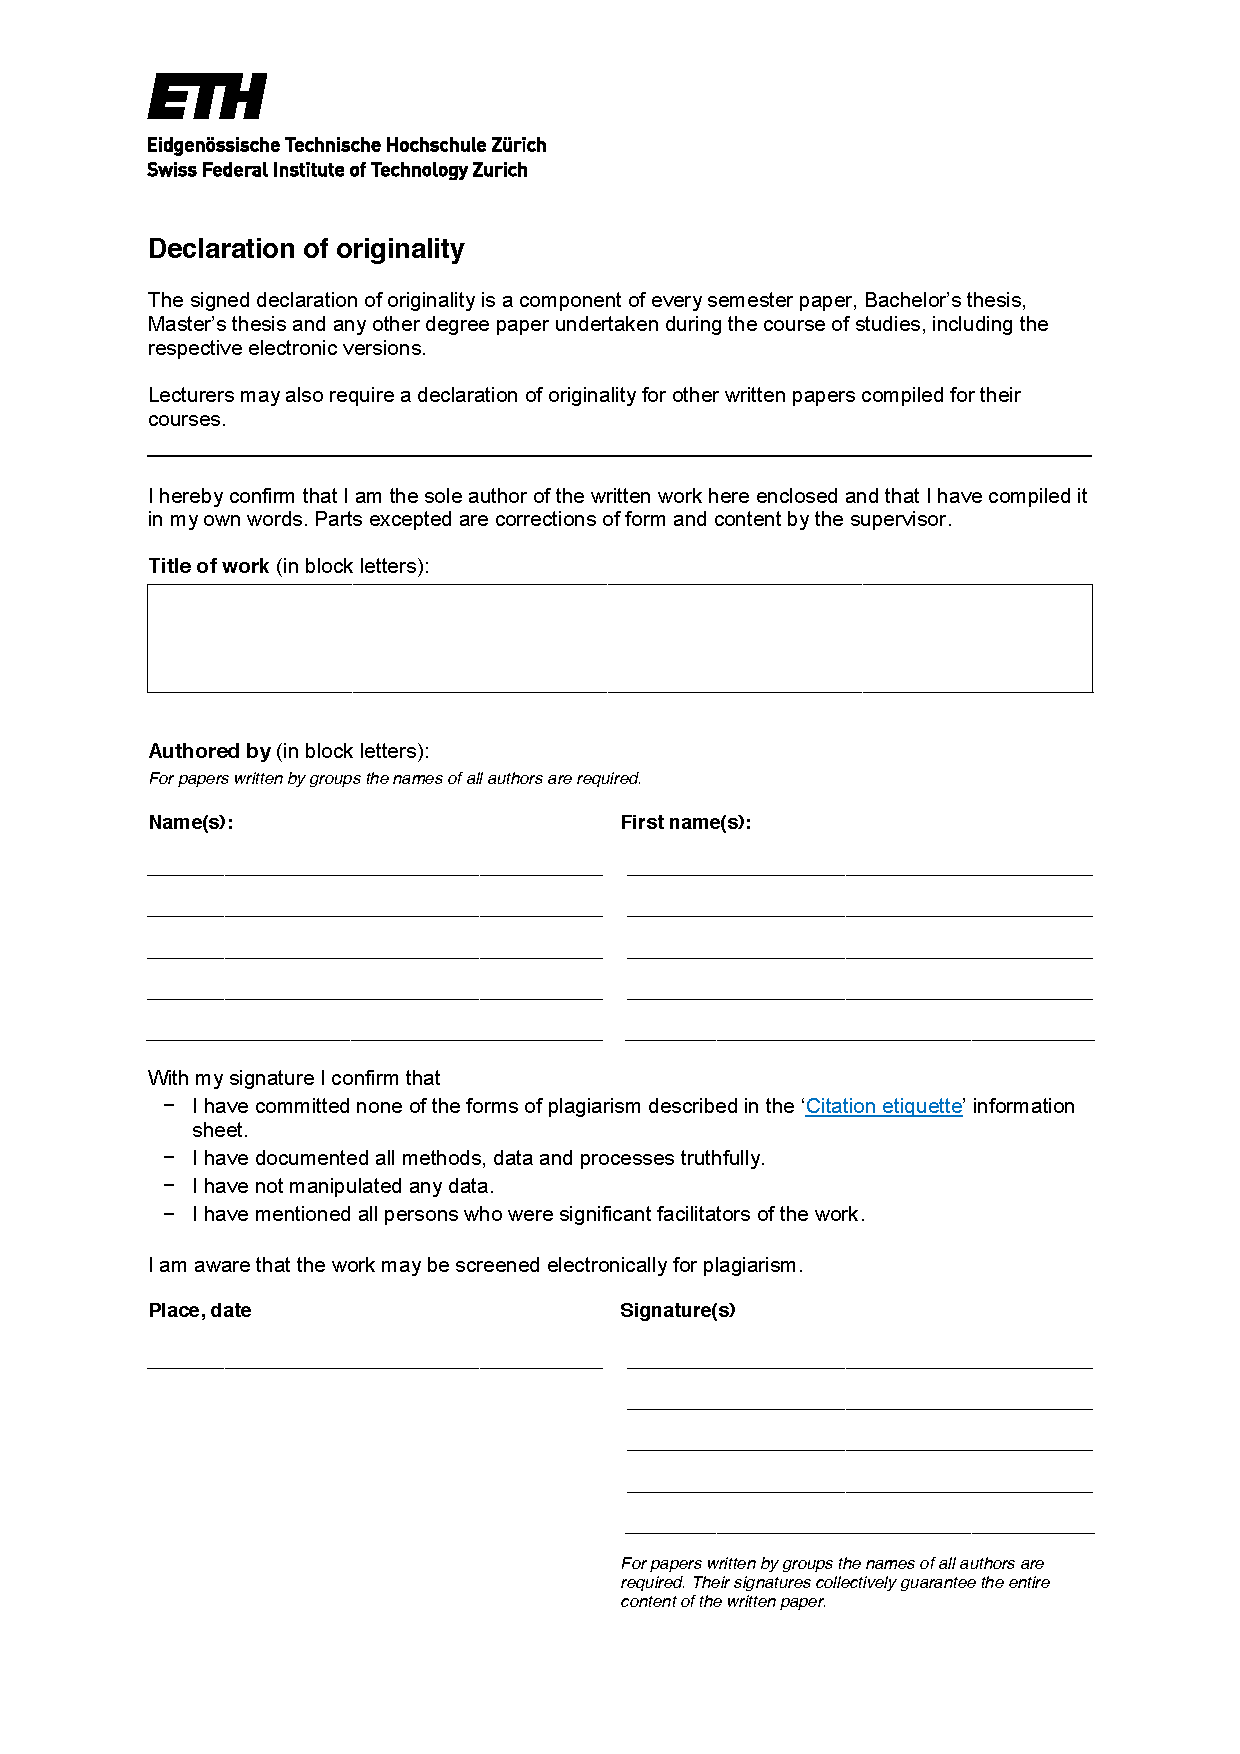
\includepdf[pages={-}]{declaration-originality.pdf}

\end{document}
